\subsection{Preemptible functions: \textit{libinger}}
\label{sec:libinger}

Our primary deliverable is the libinger library that exposes our interface.  In order
to provide an API centered around familiar function calls that adhere to the standard
stack discipline, the library hides a lot of internal unstructured control flow.
When \texttt{launch()} and \texttt{resume()} are executing the user-provided
function, they use a signal handler to asynchronously monitor its execution time.  If
it exceeds its timeout, they must context switch back to the caller, returning a
continuation that stores the preemptible function's register values.  Furthermore,
because the continuation might later be resumed, \texttt{launch()} cannot allow the
caller's intervening code to clobber the stack frames left behind by preemption, and
must therefore invoke the user function on a separate execution stack.  The library
implements all of these steps in userland.

Although seeking to implement low-latency preemption without requiring a custom
operating system, we informed our design decisions by consulting the Shinjuku
authors' study comparing the latency of bare-metal interprocessor interrupts (IPIs)
against that of Linux signals (measured from their request by one core to the
invocation of the other's interrupt service routine or signal handler).  While their
results show that IPIs take an average of only 1993 cycles, compared to 4950 for
signals (a ratio of 1:2.5), a look at their sender/receiver breakdown of the latter
number suggests two opportunities for measurable reductions to this overhead without
eschewing the existing systems software stack:  First, 343 of those cycles (6.9\%)
are spent propagating the signal between the two cores, and should largely disappear
by initiating it on the same thread that is to be preempted.  Second, 2084 cycles
(42\%) are incurred by the sender, of which some portion should also
disappear~\cite{Kaffes:nsdi2019}.  We therefore expect that an optimized system based
on intra-thread signals and built atop the existing system stack could achieve an
average preemption latency overhead slower than that of their custom operating
system with a dedicated watchdog core by a factor less than 2.5.

We base our preemption mechanism on that employed by RT, which uses a POSIX timer to
repeatedly trigger their \texttt{RELEASE\_SIGNAL}, whose handler forwards the
notification to other worker threads by \texttt{kill()}'ing them with a second
signal, \texttt{PREEMPTION\_SIGNAL}~\cite{mollison:rtas2013}.  To avoid the sender
overhead, we need to eliminate the two-phase signaling, ideally by just subscribing
each thread to the same \texttt{RELEASE\_SIGNAL}.  Unfortunately, according to the
Linux Programmer's Manual~\cite{signal-manpage}, ``A process-directed signal may be
delivered to any one of the threads that does not currently have the signal blocked.
If more than one of the threads has the signal unblocked, then the kernel chooses an
arbitrary thread to which to deliver the signal.''  We work around this limitation by
configuring a different POSIX timer with its own signal for each thread that is
currently executing a preemptible function.  All threads use the same handler, but
store their preemption signal in a thread-local variable.  Whenever the handler runs,
it checks whether it was triggered by the current thread's signal.  If not, it masks
the rogue signal and immediately returns; in this way, the system quickly converges
on delivering each preemption signal only to its corresponding thread.  The current
implementation sets each timer to fire at a fixed scheduling interval in the tens of
microseconds\footnote{The efficiency of long-running preemptible functions could be
improved with relative ease by delaying the start of these periodic signals until
hundreds of microseconds before the timeout was hit; in this way, most of long
functions' execution time would run without any throughput degradation, yet their
preemption could still be quite accurate (free of warmup effects).}.

Figure~\ref{fig:callsimple} shows what happens on each call to the \texttt{launch()}
function.  We create a \textbf{checkpoint} continuation using the POSIX
\texttt{getcontext()} function; this will be needed in the event the preemptible
function times out.  Next, we allocate a fixed-size execution stack and switch to it
using the \texttt{makecontext()} and \texttt{setcontext()} functions.  Then, if the
current thread doesn't already have a preemption signal assigned, we allocate one
from a pool of rarely-used signal numbers.  Finally, we configure a POSIX timer via
\texttt{timer\_settime()} and call the user-provided preemptible funcion.

\begin{figure}
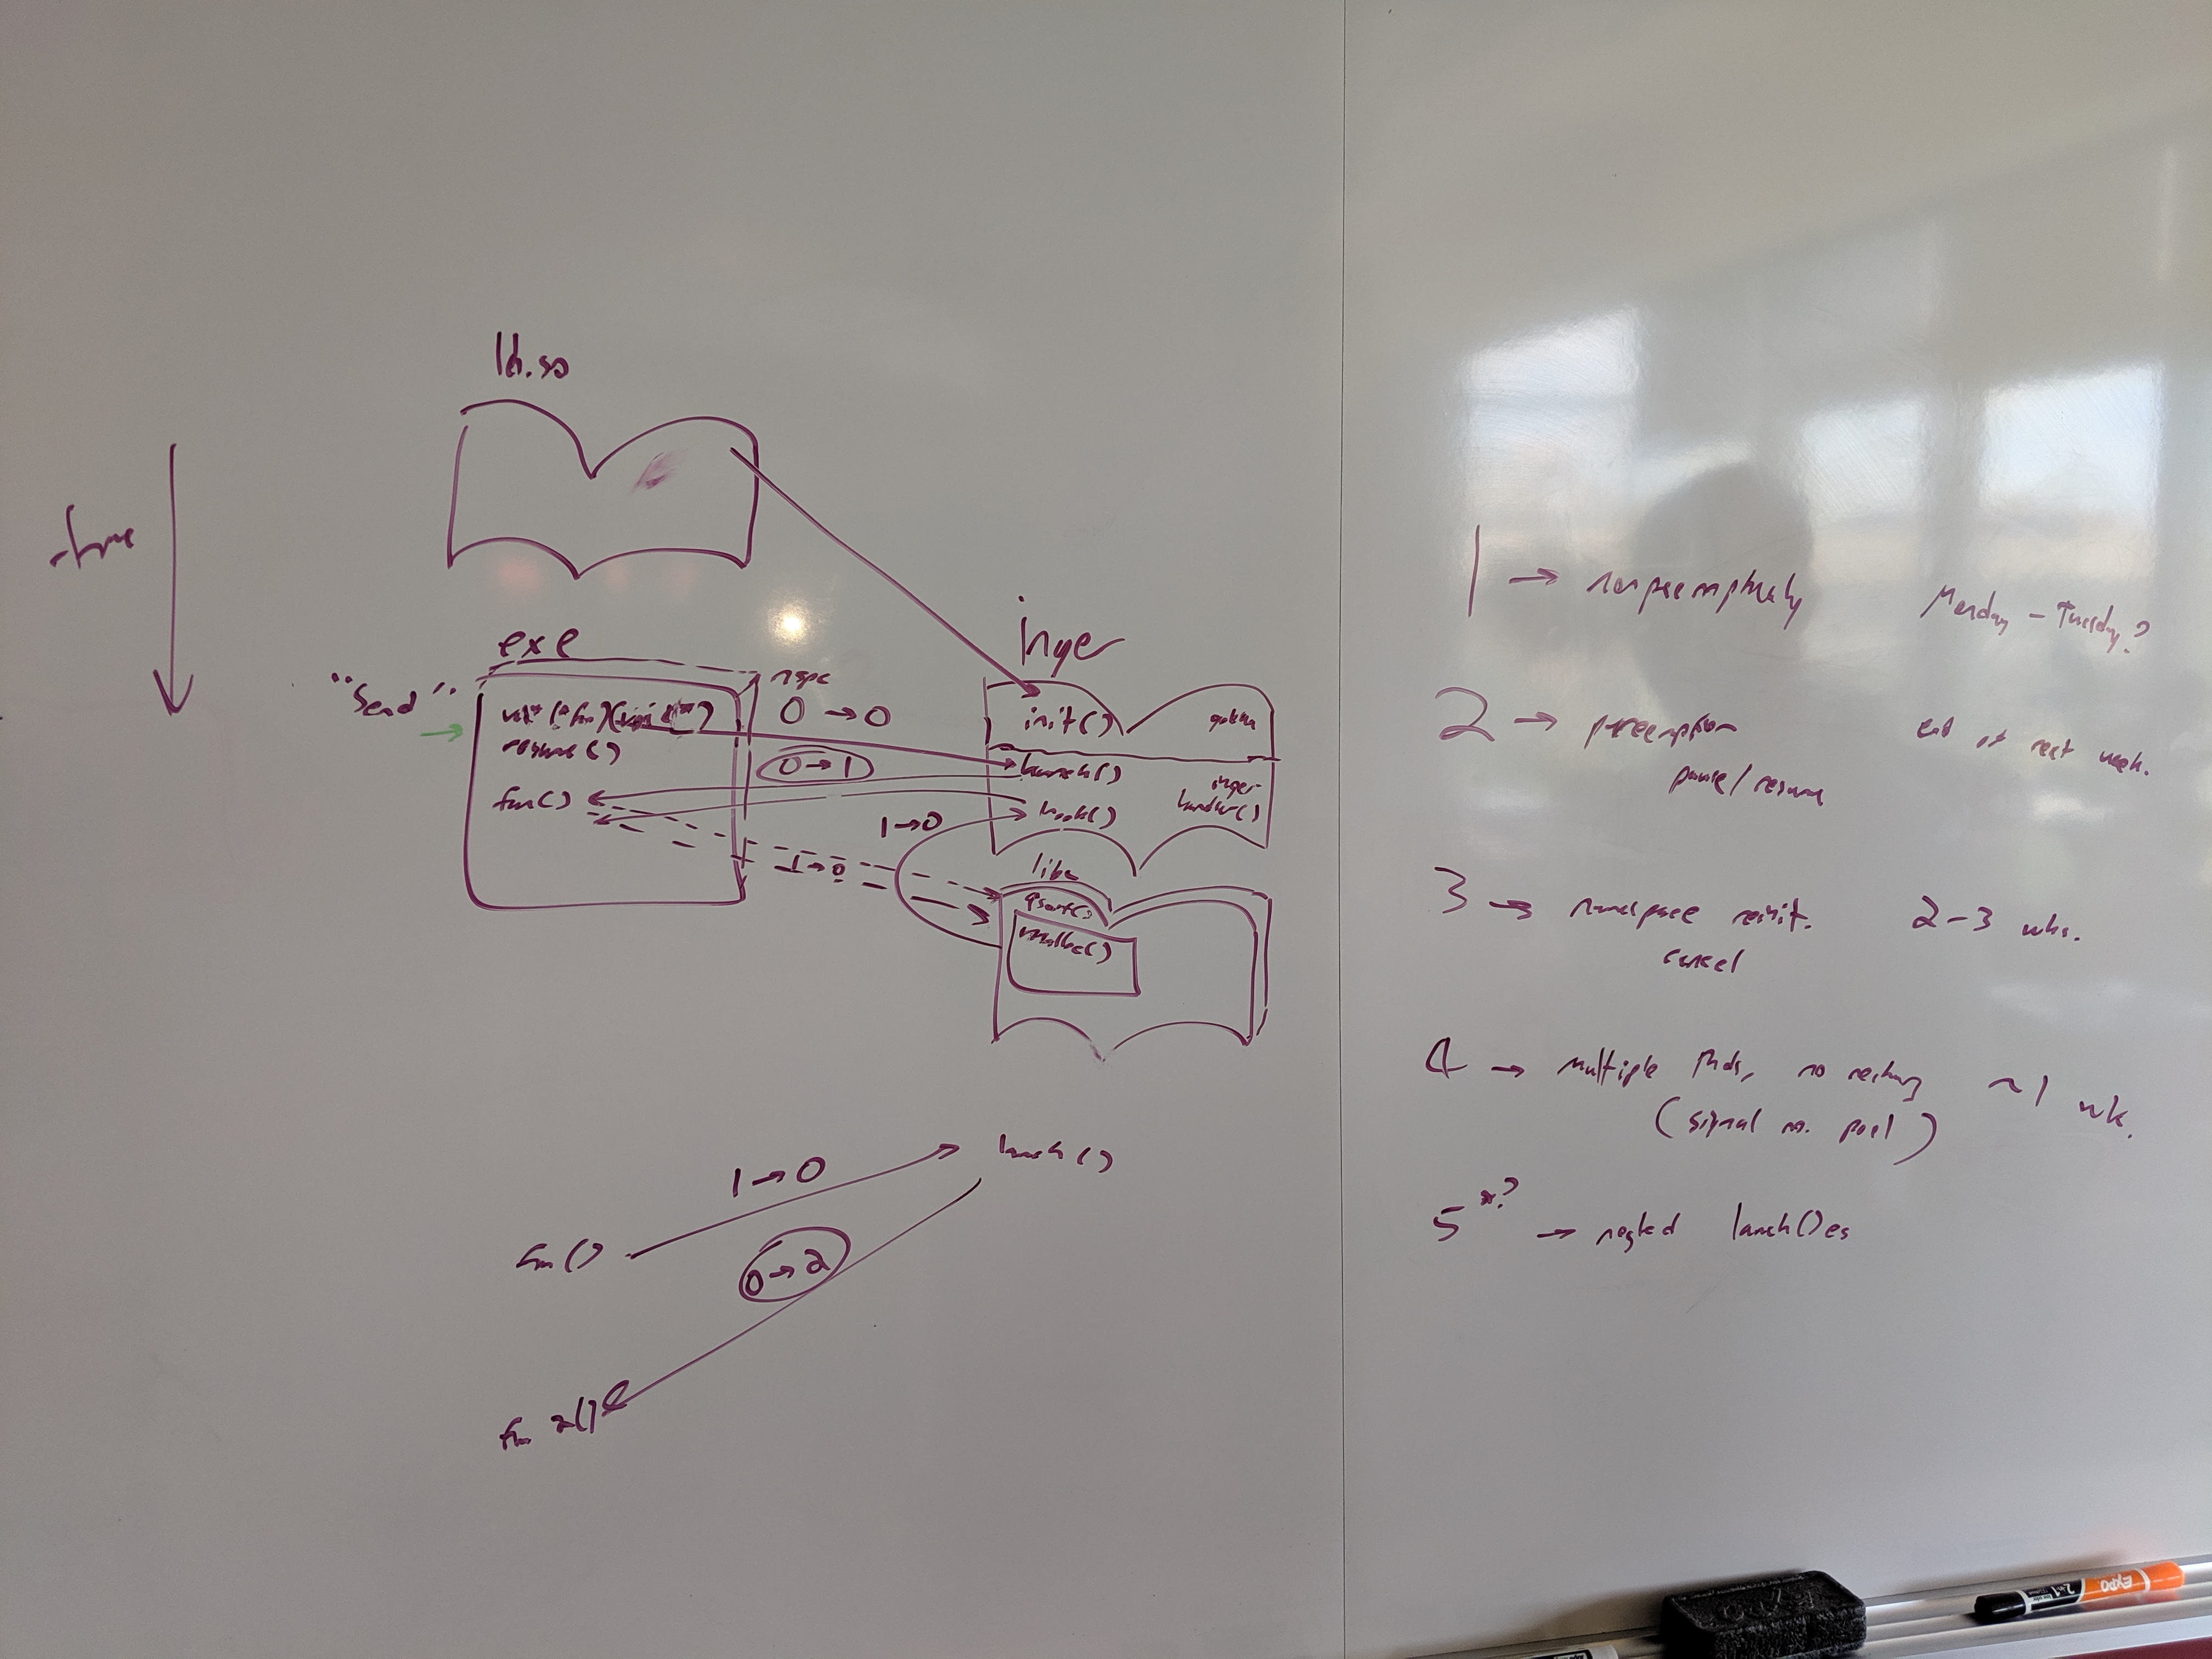
\includegraphics[width=\columnwidth]{figs/calltree}
\caption{How preemptible function dispatch works}
\label{fig:callsimple}
\end{figure}

While the preemptible function is running, the POSIX timer fires periodically,
causing a signal handler to be invoked each time.  Figure~\ref{fig:twostacks} shows
the two stacks of execution present while the handler is running, as well as what
happens to the stack frames of both if the function times out.  The handler first
checks whether the preemption signal was intended for the current thread, as
described earlier.  It then checks whether the preemptible function has exceeded its
timeout; if so, it swaps the contents of the signal handler's continuation
(accessible via the final argument to the function~\cite{sigaction-manpage}) with the
checkpoint continuation saved by \texttt{launch()}.  This causes the subsequent
return from the signal handler to jump back to \texttt{launch()}, which then returns
a \texttt{linger} structure containing the signal handler's original context.  A
subsequent \texttt{resume()} call on this packaged continuation proceeds in much the
same way as \texttt{launch()}, but resumes the original computation by sending itself
a special signal with \texttt{pthread\_kill()}, then swapping the saved context with
the contents of that handler's context.

\begin{figure}
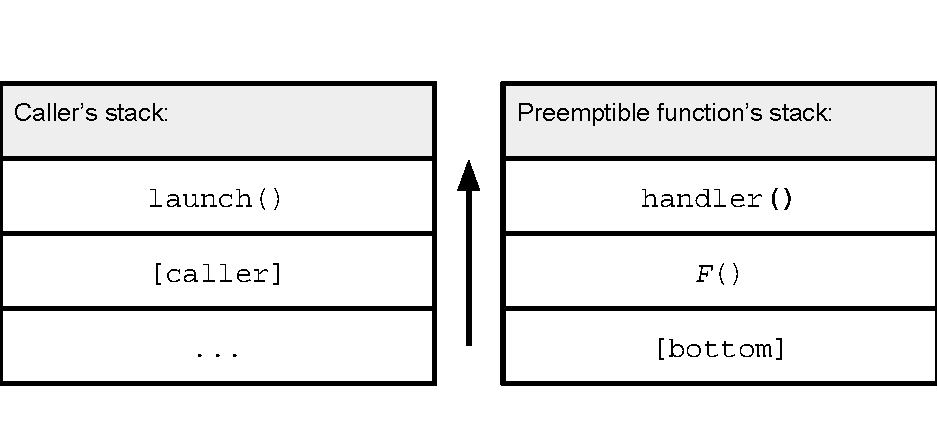
\includegraphics[width=\columnwidth]{figs/twostacks}
\caption{The two stacks before and after a timeout.  \textnormal{Upon discovering
that the preemptible function has exceeded its time bound, the handler returns to the
checkpoint continuation within the \texttt{launch()} function, removing its own stack
frame in the process.  Then, \texttt{launch()} returns to the original call site,
which removes its stack frame.}}
\label{fig:twostacks}
\end{figure}

When the caller is finished with a deallocator, it must deallocate it either
explicitly (C) or implicitly via the \texttt{inger} type's destructor (Rust).  This
cleans up the libinger resources allocated by \texttt{launch()}; however, the
current implementation of libinger does not automatically clean up resources
allocated by preemptible functions that are canceled.  While this is inherently hard
to do in C, it is possible to implement in languages such as Rust that support
destructors.  For instance, the approach proposed by Boucher et
al.~\cite{boucher:atc2018} could be employed to raise a panic (exception) on the
preemptible function's stack, causing the language runtime to unwind each stack frame,
invoking the destructor of each local variable in the process.

\subsection{Case study: Userland threading}
\label{sec:threading}
